\documentclass[12pt, preprint]{aastex}
%\usepackage{bm, graphicx, subfigure, amsmath, morefloats}
\bibliographystyle{apj}
\usepackage{float, bm, graphicx, subfigure, amsmath, morefloats}
\usepackage{color}
\usepackage{caption}
\usepackage{subcaption}

% naming macros
\newcommand{\tc}{\textsl{The~Cannon}} 
\newcommand{\cannon}{\textsl{Cannon}} 
\newcommand{\apogee}{\textsl{APOGEE}} 
\newcommand{\aspcap}{\textsl{ASPCAP}}
\newcommand{\lamost}{\textsl{LAMOST}}
\newcommand{\segue}{\textsl{SEGUE}}
\newcommand{\rave}{\textsl{RAVE}}
\newcommand{\galah}{\textsl{GALAH}}
\newcommand{\gaiaeso}{\textsl{Gaia-ESO}}
\newcommand{\kepler}{\textsl{Kepler}}
\newcommand{\ulyss}{\textsl{ULySS}}

% math and symbol macros
\newcommand{\set}[1]{\bm{#1}}
\newcommand{\teff}{\mbox{$\rm T_{eff}$}}
\newcommand{\feh}{\mbox{$\rm [Fe/H]$}}
\newcommand{\alphafe}{\mbox{$\rm [\alpha/Fe]$}}
\newcommand{\mh}{\mbox{$\rm [M/H]$}}
\newcommand{\logg}{\mbox{$\rm \log g$}}
\newcommand{\cm}{\mbox{$\rm [C/M]$}}
\newcommand{\nm}{\mbox{$\rm [N/M]$}}
\newcommand{\starlabel}{\ell}
\newcommand{\starlabelvec}{\set{\starlabel}}
\newcommand{\given}{\,|\,}
\newcommand{\ntestobj}{448,903}

\begin{document}

\title{Survey Cross-Calibration Using \tc: \\ \apogee\ Labels from \lamost\ Spectra}
\author{A. Y. Q. ~Ho\altaffilmark{1},
M.~Ness\altaffilmark{1},
David~W.~Hogg\altaffilmark{1,2,3}, 
H.-W.~Rix\altaffilmark{1},
M.~Fouesneau\altaffilmark{1},
C.~Liu\altaffilmark{4},
F.~Yang\altaffilmark{4}
}
\altaffiltext{1}{Max-Planck-Institut f\"ur Astronomie, K\"onigstuhl 17, D-69117 Heidelberg, Germany}
\altaffiltext{2}{Center for Cosmology and Particle Physics, Department of Phyics,
New York University, 4 Washington Pl., room 424, New York, NY, 10003, USA}
\altaffiltext{3}{Center for Data Science, New York University, 726 Broadway, 7th Floor, New York, NY 10003, USA}
\altaffiltext{4}{Key Laboratory of Optical Astronomy, National Astronomical Observatories, Chinese Academy of Sciences, Datun Road 20A,Beijin 100012, China}

\email{annaho@mpia.de}

\begin{abstract}

To capitalize on the new generation of large spectroscopic stellar surveys, 
it is essential to develop robust methods for cross-calibration; that is, for putting 
qualitatively different surveys onto the same physical parameter and chemical
abundance (collectively ``stellar label") scale. In this work, we demonstrate that
cross-calibration can be achieved using \tc\ \citep{ness2015}, a new data-driven
approach to determining stellar labels from stellar spectra. 
In particular, we bring the \apogee\ and \lamost\ surveys onto the \apogee\
scale by using the 11,057 objects observed in common between the
two surveys as ``reference objects" to fit for a spectral model that 
maps \lamost\ stellar spectra to four corresponding \apogee\ labels: 
\teff, \logg, \feh, and \alphafe. 
We apply this model to the \lamost\ spectra for the 11,057 training objects
and infer labels that are consistent with the \apogee\ labels within 
the stated \aspcap\ uncertainties, thus correcting the existing bias between labels 
derived from \apogee\ spectra and those derived from \lamost\ spectra. 
We then apply the model to determine \apogee-scale labels for 
\ntestobj\ giants in \lamost\ DR2 that were \emph{not} 
observed with \apogee, and in doing so perform the first-ever
\alphafe\ measurement from \lamost\ 
spectra. Thus, we demonstrate that \tc\ can not only be used to put
spectroscopic stellar surveys onto the same physical scale, but also to
``transfer" labels from one survey to another. 

\end{abstract}

\keywords{
methods: data analysis
---
methods: statistical
---
stars: abundances
---
stars: fundamental parameters
---
surveys
---
techniques: spectroscopic
}

\section{Introduction: \tc\ in the Context of Survey Cross-Calibration}

A diverse suite of large-scale stellar spectroscopic surveys
(e.g. 
\apogee\ \citep{Majewski2012},
\gaiaeso\ \citep{Gilmore2012},
\galah\ \citep{Freeman2012},
\lamost\ \citep{Newberg2012},
\rave\ \citep{Steinmetz2006}, and
\segue\ \citep{Beers}
)
have been measuring spectra for hundreds of thousands of stars in the Milky Way. 
In a few years, thanks to Gaia, these spectra will number in the hundreds of millions. 
That these surveys are diverse in focus (e.g. in which stellar populations
they target) holds promise for a more complete understanding of the galaxy. 
That they are technically diverse (e.g. in 
wavelength coverage and resolution) presents a challenge,
because forming a complete picture necessites stitching data from 
these surveys together. 
That cannot be done at present, because spectroscopic analysis pipelines
are customized to individual survey properties such that different 
pipelines measure substantially different properties for the same stars 
(e.g. \citet{Smiljanic2014}). 
Thus, techniques need to be developed for survey cross-calibration: 
for bringing physical parameters and chemical
abundances (collectively ``stellar labels") from different surveys 
onto a single physical scale. 

\tc\ \citep{ness2015} is a new data-driven method for measuring stellar labels 
from spectra in the context of large spectroscopic surveys. \citet{ness2015} 
describe the method and its application to \apogee\ DR10 spectra in detail,
and highlight its potential for performing survey
cross-calibration. Here, we recapitulate the fundamental assumptions and steps
of \tc\ in the context of survey cross-calibation. 

\tc\ makes two assumptions: that the spectra of stars with identical labels look identical,
and that spectra vary smoothly with label changes. In other words, the continuum-normalized flux at each pixel in the spectrum is a smooth function of the labels. The function
that maps the flux in a single pixel of an object's spectrum to that object's labels 
is called the ``spectral model." 

Presume that we would like to use \tc\ to cross-calibrate Survey A and Survey B,
which have some set of objects measured in commn. 
For each survey, we have a set of spectra measured by that survey 
and a set of labels measured by that survey's pipeline; 
for example, from Survey A we have spectra measured
by Survey A and labels measured by Survey A's pipeline. 
The surveys are not yet on the same label scale; that is,
for a single object measured in common between the surveys, 
the Survey A and Survey B pipelines measure inconsistent labels. 

Presume further that we trust Survey A's labels more than Survey B's, 
so we decide to cross-calibrate
by bringing Survey B onto Survey A's label scale. That is, for an object
measured in common between the surveys, our Cannon pipeline
should measure Survey A labels from the Survey B spectrum that are
consistent with Survey A labels measured from the corresponding 
Survey A spectrum using the Survey A pipeline. 

To accomplish this, \tc\ proceeds in two steps: 
a ``training step" and then a ``test step." 
In the training step, \tc\ uses the objects measured
in common between the two surveys as ``reference objects"
to fit for a spectral model at each pixel of the spectrum independently. 
More precisely, the model characterizes each pixel of a Survey B 
spectrum as a function of corresponding Survey A labels. 
In the test step, the spectral model is applied to each of the remaining objects
in Survey B (those not observed by Survey A) to infer their Survey A-scale labels.
Note that all of the reference \emph{spectra} come from Survey B, 
and all of the reference \emph{labels} come from Survey A; thus, 
if the Survey A pipeline has measured a dozen labels precisely and the 
Survey B pipeline has only measured three, we can in principle use
our model to infer extra, previously unknown labels from Survey B spectra. 
We dub this process of transferring knowledge of labels from one survey
to another ``label transfer." 

In this work, Survey A is \apogee\ and Survey B is \lamost. 
In other words, we use \tc\ to cross-calibrate the \apogee\
and \lamost\ surveys by measuring four \apogee-scale labels
(\teff, \logg, \feh, and \alphafe)
directly from \lamost\ spectra. We choose the \apogee\ label
scale because it is the higher-resolution survey ($R\approx22,500$
versus $R\approx1,800$ for \lamost).

The reference objects are thus the 11,057 objects
measured in common between these two surveys, and the training step consists
of using these objects to fit for a spectral model that maps each pixel of
a normalized \lamost\ spectrum to the corresponding \apogee\ labels 
\teff, \logg, \feh, and \alphafe. 
The test step consists of applying this spectral model to the remaining
\lamost\ objects in DR2 not measured by \apogee\ ($\approx\,500,000$ giants)
and inferring their \apogee-scale labels. 

The code used in this work is an implementation of the procedure outlined in 
\citet{ness2015}. The primary difference between this procedure and the one used
in \citet{ness2015} is in how the spectra were continuum normalized; we
describe that process in Section \ref{sec:data}. 

\section{Data: \lamost\ and \apogee}\label{sec:data}

The Large sky Area Multi-Object Spectroscopic Telescope (\lamost) 
is a low-resolution ($R\approx1,800$) optical ($3650-9000\,\mbox{\AA}$) 
spectroscopic survey.
As of the second data release (DR2; \citet{Luo2015}) \lamost\ has 
measured spectra for $\approx 4,136,000$ objects and 
three stellar parameters (\teff, \logg, \feh) for $\approx 2,200,000$ stars. 
Parameters are derived by
the package \ulyss\ \citep{Wu2011} which calculates the fit between each spectrum and a 
model spectrum. The model spectrum is a linear combination of non-linear components,
optically convolved with a line-of-sight velocity
distribution and multiplied by a polynomial function. 

\apogee\ is a high resolution ($R\approx22,500$) high SNR ($SNR\approx100$) 
H-band (15200-16900\,$\mbox{\AA}$) spectroscopic survey of 
primarily red giants spanning the bulge, disk, and MW halo \citep{Zaso2013}.
As of the most recent release (DR12, released as part of the 12th data release
of the Sloan Digital Sky Survey; \citet{Majewski2015}, \citet{Eisenstein2011}) 
\apogee\ has measured spectra
for 100,000 red giant stars as well as three parameters and 15 chemical
abundances for each star. The parameters and abundances are 
derived by the ASPCAP pipeline, which is based on chi-sq fitting of
the data to 1D LTE models for seven labels (\teff, \logg, \feh, \alphafe, \cm, \nm, 
and micro-turbulence; Garcia Perez et al. 2015, in prep). 

\section{Preparing Data for \tc} 

Before being fed to \tc, any spectroscopic data set must satisfy the criteria laid out in 
\citet{ness2015}. More specifically, the spectra must be normalized in a consistent way
that is independent of S/N, must share a
common line-spread function, and must be radial velocity shifted and sampled onto
a common wavelength grid. The flux at each pixel of each spectrum must be accompanied
by a flux variance that takes error sources such as photon noise and poor sky subtraction
into account. 

Raw \lamost\ spectra do not satisfy these criteria, so we had to process the
spectra using the following steps. First, the displacement from the rest frame was
calculated for each spectrum using the redshift value provided in 
the data file header. This caused the spectra to be on different 
wavelength grids, so we resampled each spectrum through interpolation
onto the original grid. The lower and upper limits of the spectra were 
not consistent, so we applied cuts such that the lower and upper 
wavelengths were 3900\,$\mbox{\AA}$ and 8800\,$\mbox{\AA}$ respectively.
All of these operations were performed on the flux as well as inverse variance
arrays. 

The spectra were then normalized by \tc. 
This was not true ``continuum normalization;" rather, the goal was to remove
the overall shape of the spectrum resulting from instrument effects. 
First, a smoothed version of each spectrum was calculated using a running Gaussian. 
The smoothed
flux at wavelength $\lambda_0$, $\bar{f} (\lambda_0)$ was thus:

\begin{equation}
\bar{f}(\lambda_0) = \frac{\sum_i (f_i\,\sigma^{-2}_i\,w_i(\lambda_0))}{\sum_i (\sigma^{-2}_i\,w_i(\lambda_0))}
\end{equation}

\noindent where $f_i$ is the flux at pixel $i$, $\sigma_i$ is the uncertainty at pixel $i$, 
and $w_i (\lambda_0)$ is the weight at pixel $i$ drawn from a Gaussian distribution 
centered at $\lambda=\lambda_0$. In other words, 

\begin{equation}
w_i(\lambda_0) = e^{-\frac{(\lambda_0-\lambda_i)^2}{L^2}}
\end{equation}

\noindent We chose $L$ to be equal to 50\,$\mbox{\AA}$ in order to avoid 
smearing out atomic lines. The normalized flux at each pixel was the 
original flux divided by the smoothed value. 
A sample training set spectrum with its \apogee\ spectrum, its 
\lamost\ spectrum and Gaussian-smoothed ``continuum," 
and final ``normalized" \lamost\ spectrum is shown in 
Figure \ref{fig:sample_spec}. 

\begin{figure}[h!]
\centering
\includegraphics[scale=0.8]{sample_spec.png}
\caption{(Top) The \apogee\ spectrum for a sample training objects,
(Middle) the corresponding \lamost\ spectrum for that object overlaid
with the Gaussian-smoothed ``continuum," and (Bottom) the 
resulting ``continuum-normalized"
\lamost\ spectrum used as input to \tc}
\label{fig:sample_spec}
\end{figure}

\section{\tc\ Training Step: \\ Use Reference Objects to Fit a Spectral Model}

Our reference set comprises the 11,057 objects measured in common between
\lamost\ DR2 and \apogee\ DR12. 
For the training step, It is essential for the reference set to have trustworthy labels, 
so we cut out objects with unreliable \teff, \logg, \feh, and \alphafe\ as laid out in 
\citet{Holtzman2015} and on the \apogee\ DR12 website. We use the 
following criteria for unreliable labels: $4000 < \teff < 6000$, $\logg < 0$,  
the flags \texttt{STAR\_WARN}, \texttt{M\_H\_WARN}, \texttt{ALPHAFE\_WARN}, and individual
element flags for \teff, \logg, \feh, and \alphafe. 
After applying these cuts, 9339 of the 11,057 overlap objects remained. 

The location of the training set in \lamost\ \teff-\logg\ label space is shown in 
Figure \ref{fig:training-set-label-space}. The training objects (colored points)
are overlaid on top of the full \lamost\ DR2 sample (black points). Note
that these label values are the \lamost\ label values, not the \apogee\ label
values used in training. 

\begin{figure}[h!]
\centering
\includegraphics[scale=0.58]{ts_in_full_lamost_label_space.png}
\caption{(Black) all LAMOST DR2 points in \teff-\logg\ space, with (Color) training set overlaid}
\label{fig:training-set-label-space}
\end{figure}

\tc\ uses the reference objects to fit for a spectral model that characterizes the flux
in each pixel of the (normalized) spectrum as a function $g$ of the labels of the star. 
In general, the flux $f$ for object $n$ at wavelength $\lambda$ can be written as

\begin{eqnarray}
f_{n\lambda} &=&
g(\starlabelvec_n |  \set{\theta}_\lambda) + \mbox{noise}
\label{eq:specmodel}\quad 
\end{eqnarray}

\noindent where $\set{\theta}_\lambda$ is the set of 
spectral model coefficients at each wavelength of the spectrum $\lambda$ and
$\starlabelvec_n$ is some (possibly complicated) function of the full set of labels. 
The noise model is $\mbox{noise} = [s_\lambda^2+ \sigma_{n\lambda}^2]\,\xi_{n\lambda}$,
where each $\xi_{n\lambda}$ is a Gaussian random number with zero mean and unit
variance.The noise is thus an $rms$ combination of inherent uncertainty in the spectrum
from e.g. instrument effects and finite photon counts ($\sigma_{n\lambda}$) and 
intrinsic scatter in the model at each wavelength ($s_\lambda$). 
The way we handle uncertainties - by fitting for a noise model
independently at each pixel - is a key feature of \tc\ and is what 
distinguishes it from traditional machine learning
methods. 

Following \citet{ness2015} we presume that the model $g$ can be written 
 as a linear function of $\starlabelvec_n$: 

\begin{eqnarray}
f_{n\lambda} &=&
\set{\theta}_\lambda^T \cdot \starlabelvec_n + \mbox{noise}
\label{eq:linearmodel}\quad
\end{eqnarray}

\noindent corresponding to the single-pixel log likelihood function

\begin{eqnarray}
\ln p(f_{n\lambda}\given\set{\theta}^T_\lambda, \starlabelvec_n, s_\lambda^2) &=&
 -\frac{1}{2}\,\frac{[f_{n\lambda} - \set{\theta}^T_\lambda \cdot \starlabelvec_n]^2}{s_\lambda^2 + \sigma_{n\lambda}^2}
 -\frac{1}{2}\,\ln(s_\lambda^2 + \sigma_{n\lambda}^2)
\label{eq:like}\quad.
\end{eqnarray}

\noindent For this work, once more as in \citet{ness2015}, 
we use a quadratic model such that $\starlabelvec_n$ is  

\begin{equation}
\begin{split}
\starlabelvec_n \equiv [1, \teff, \logg, \feh, \alpha, \teff^2, \teff\cdot\logg, \teff\cdot\feh, \teff\cdot\alpha, \\
\logg^2, \logg\cdot\feh, \logg\cdot\alpha, \feh^2, \feh\cdot\alpha, \alpha^2]
\label{eq:quadinthreelabels}
\end{split}
\end{equation}

The training step thus consists holding the labels in the label vector 
$\starlabelvec_n$ as fixed (these are the training labels) and optimizing the 
log likelihood to solve for the coefficients 
$[\theta_\lambda, s_\lambda^2]$ independently at every pixel. 
For a fixed scatter, optimization is a pure linear-algebra operation
(weighted least squares). Currently, we optimize for the scatter by stepping through
a grid of scatter values. 

Figure \ref{fig:leading-coeffs} shows the leading (linear) coefficient for each label as
a function of wavelength, as well as the scatter as a function of wavelength.
The magnitude of the leading coefficient can be thought of as a proxy for how 
sensitive a particular pixel is to that particular label. Thus, Figure \ref{fig:leading-coeffs}
is a way to visualize which pixels in the spectrum are determined by \tc\ to be
important for which labels. It makes sense, therefore, that peaks in these coefficients
correspond to well-known spectral lines such as the calcium triplet. 

\begin{figure}[h!]
\centering
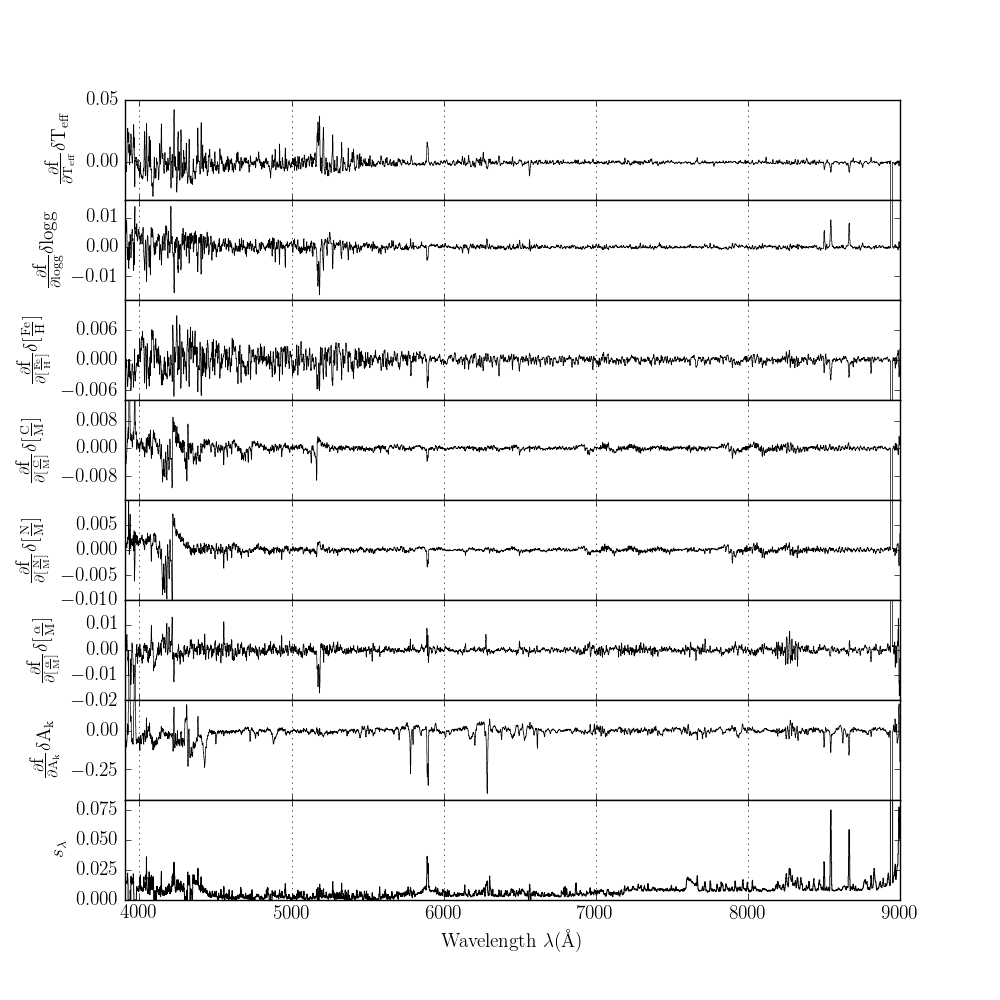
\includegraphics[scale=0.8]{leading_coeffs.png}
\caption{Leading (linear) coefficients and scatter from the spectral model fit to the 9339 reference objects. These leading coefficients indicate how sensitive each pixel in the spectrum is to each of the labels.}
\label{fig:leading-coeffs}
\end{figure}

\section{\tc\ Test Step: \\ Use the Spectral Model to Infer Labels for Test Objects}

In the training step, we held the labels in $\starlabelvec_n$ fixed and 
solved for the coefficients of the spectral model. 
Now, in the test step, we now hold the spectral model coefficients fixed 
and solve for the labels in $\starlabelvec_n$ for each test object $n$. 
For a model that is quadratic in the labels, like ours, this consists of 
non-linear optimization; we use Python's curve fit routine. 

\citet{Chen2015} compared the three stellar parameters \teff, \logg, and 
\feh\ between \apogee\ and \lamost\ and found close consistency in \teff\
but systematic biases in \logg\ and \feh. Figure \ref{fig:apogee-lamost} 
shows the comparison for these three parameters for all 9339 objects in 
the reference set. After training, we have a model that characterizes the flux 
in each \lamost\ spectrum as a function of four \apogee\ labels. 
To test our model, we feed the 9339 reference objects back into \tc\ as 
test objects, to see whether we can infer \apogee-scale labels directly from
\lamost\ spectra. The results are new Cannon-\lamost\ labels: labels measured
by \tc\ from \lamost\ spectra. Figure \ref{fig:apogee-cannon} shows these labels
plotted against the corresponding \apogee\ labels. A direct comparison of
Figures \ref{fig:apogee-lamost} and \ref{fig:apogee-cannon} shows significant
improvement in scatter and bias, particularly in \logg\ and \feh, showing that
we have successfully measured \apogee-scale and not \lamost-scale labels 
directly from \lamost\ spectra. 

\begin{figure}[h!]
\centering
\includegraphics[scale=0.6]{apogee_lamost.png}
\caption{Comparison of \teff, \logg, and \feh\ for all 9339 in the training set (overlap
objects between \lamost\ and \apogee). There are clear systematic biases in \logg\
and \feh.}
\label{fig:apogee-lamost}
\end{figure}

\begin{figure}[h!]
\centering
\includegraphics[scale=0.6]{apogee_cannon.png}
\caption{Comparison between Cannon-\lamost\ (measured by \tc\ from \lamost\ spectra) and \apogee\ \teff, \logg, and \feh\ for all 9339 in the training set (overlap
objects between \lamost\ and \apogee). The biases in \logg\
and \feh\ from Figure \ref{fig:apogee-lamost} have been significantly reduced.}
\label{fig:apogee-cannon}
\end{figure}

The next step is to apply the spectral model to DR2 objects that were \emph{not}
measured by \apogee. We could not blindly apply the spectral model to all 
DR2 objects; as shown
in \citet{ness2015}, \tc\ becomes less reliable with increasing distance from
the label space of the reference set. Thus, for our test set we had to select
DR2 data that was sufficiently close to the reference label space of the 
\apogee-\lamost\ overlap objects. 
We applied a cut based on the 
distance of the test object's \lamost's values from the reference label space. 
We define the ``distance" between a point in \lamost\ label space (indicated
by the subscript $L$) and a point in \apogee\ label space (indicated by the
subscript $A$) to be

\begin{equation}
D = \frac{1}{K_{\teff}^2} (\teff_{,L}-\teff_{,A})^2 + 
\frac{1}{K_{\logg}^2} (\logg_{L}-\logg_{A})^2 + 
\frac{1}{K_{\feh}^2} (\feh_{L}-\feh_{A})^2 
\end{equation}

\noindent where $K_{\teff}=100$, $K_{\logg}=0.20$, $K_{\feh}=0.10$, corresponding to the 
approximate uncertainty in each label. The distance from any given candidate test object to
the reference label space was calculated as the average of its distances to the ten
nearest reference objects. 

Our distance cut (the distance within which a \lamost\ DR2 object was deemed a suitable
test object) was determined by running the test step of \tc\ through 3,000 objects in
\lamost\ DR2, all from one date (2012-11-25). In Figure \ref{fig:ts-dist} we show the distance from the resulting Cannon labels to the \lamost\ labels, 
plotted against the distance from the \lamost\ labels to the \apogee\ reference label space. 
One can see a gap between the stars corresponding to the giant branch and the stars
corresponding to the main sequence. Figure \ref{fig:ts-dist-dr2} shows all 14,000 of the stars
from this same date, overlaid on top of the same \lamost\ DR2 label space plot from Figure \ref{fig:training-set-label-space}. For the test step, we selected stars whose distance to 
reference label space was less than 2.5. 

\begin{figure}[h!]
\centering
\includegraphics[scale=0.5]{distance_comparison_colored_zoomed_labeled.png}
\caption{Giant branch stars and main sequence stars in \lamost\ DR2 separate out when their distance from reference label space is plotted against the distance from their \lamost\ labels to their Cannon labels, which are determined by running these stars through \tc\ test step.}
\label{fig:ts-dist}
\end{figure}

\begin{figure}[h!]
\centering
\includegraphics[scale=0.58]{ts_distance_in_full_lamost_label_space.png}
\caption{(Black) all LAMOST DR2 points in \teff-\logg\ space, with (Color) 14,000 objects overlaid color-coded by their distances from the training label space. For the test step, we choose objects whose distances are less than 2.5}
\label{fig:ts-dist-dr2}
\end{figure}

With the test set identified in this way, \ntestobj\ stars (giants) remained. The Cannon-\lamost\ 
labels for these objects are available in a table online and an excerpt is shown in Table \ref{tab:results}. 

\begin{table*}[!h]
\tiny{
\centering
\caption{Excerpt from the online table of stellar labels (\teff, \logg\, \feh and \alphafe) for 
\ntestobj\ stars, inferred by \tc\ from \lamost\ DR2 spectra} 
\begin{tabular}{| c | c | c |  c | c | c |  c | c | c | c | c | } 
\hline
\tiny{star ID}  & \teff\ & \logg\ & \feh\ & \alphafe\ & $\sigma$(\teff) & $\sigma$(\logg) & $\sigma$(\feh) & $\sigma$(\alphafe) & Red. $\chi^2$ \\
\tiny{LAMOST ID} & K & dex & dex & dex & K & dex & dex & dex &\\    
\hline
\tiny{spec-56800-HD115503N082638V01\_sp01-011} & 4903.4 & 3.44  & -0.32  & 0.16 & 2327 & 0.013 & 0.0037 & 0.00080 & 0.22 \\
\tiny{spec-56800-HD115503N082638V01\_sp01-076} & 4977.6  & 3.61  & 0.37  & 0.090 & 2010 & 0.0089 & 0.0027 & 0.00063 & 0.25 \\
\tiny{spec-56800-HD115503N082638V01\_sp01-089} & 4933.0  & 2.62  & -0.53 &  0.20 & 2690 & 0.012 & 0.0047 & 0.0011 & 0.37 \\
\hline
\end{tabular}
\label{tab:results} }
\end{table*}  

Until now, no \alphafe\ labels had been calculated for \lamost\ spectra.
However, because they are known for \apogee\ spectra, 
our model learned the ``mapping" between
\apogee-scale \alphafe\ and \lamost\ spectra, enabling us to effectively 
``transfer" the \alphafe\ label from \apogee\ to \lamost\ and measure
the first \alphafe\ values for these spectra. 
Figure \ref{fig:alpha-feh} shows the \alphafe-\feh\ 
plane for all \ntestobj\ \lamost\ DR2 giants. 

\begin{figure}[h!]
\centering
\includegraphics[scale=0.6]{feh_alpha_plane.png}
\caption{The \alphafe-\feh\ plane for all \ntestobj\ test objects. These are the first
\alphafe\ values measured from \lamost\ spectra.}
\label{fig:alpha-feh}
\end{figure}

\section{Discussion}

We have demonstrated that \tc\ can be used to put two qualitatively different stellar 
spectroscopic surveys onto the same label (physical parameter and chemical abundance)
scale, by training a spectral model on the set of objects observed in common between
the surveys. We used \lamost\ and \apogee\ as our example, and showed that we could
significantly reduce the discrepency between labels that were previously measured for overlap
objects using the two individual survey pipelines. By training our model to
infer \apogee\ labels directly from \lamost\ spectra, we were also able to calculate one label
(\alphafe) from \lamost\ spectra that was previously not available from the \lamost\ pipeline. 

Efforts are already underway to use \tc\ to cross-calibrate other surveys with
objects measured in common; for example, \rave-\apogee, \segue-\lamost, \galah-\apogee. 
Particularly promising is the use of overlap objects between \kepler\ and other surveys to
``transfer" the otherwise-difficult-to-measure astroseismetric age label. 
This is motivation for surveys to measure objects in common whose labels 
comprehensively span the label space of interest. 

The code used to produce the results described in this paper was written in
Python and is available online for public 
use.\footnote{\url{www.github.com/annayqho/the-cannon}}

\section{Acknowledgements}

AYQH was partially supported by a Fulbright grant through the German-American
Fulbright Commission.

The research has received funding from the European Research Council under the 
European Union's Seventh Framework Programme (FP 7) ERC Grant Agreement n.
[321035].

\begin{thebibliography}{24}
\expandafter\ifx\csname natexlab\endcsname\relax\def\natexlab#1{#1}\fi

\bibitem[Beers et al.(2006)]{Beers} Beers, T.~C., Lee, Y., 
Sivarani, T., et al.\ 2006, \memsai, 77, 1171 

\bibitem[Chen et al.(2015)]{Chen2015} Chen, Y.~Q., Zhao, G., 
Liu, C., et al.\ 2015, arXiv:1506.00771 

\bibitem[{{Eisenstein et al.}(2011)}]{Eisenstein2011} Eisenstein, D.J., Weinberg D.H., Agol E., et al. 2011, AJ 142, 72

\bibitem[{{Freeman}(2012)}]{Freeman2012}
{Freeman}, K.~C. 2012, in Astronomical Society of the Pacific Conference
  Series, Vol. 458, Galactic Archaeology: Near-Field Cosmology and the
  Formation of the Milky Way, ed. W.~{Aoki}, M.~{Ishigaki}, T.~{Suda},
  T.~{Tsujimoto}, \& N.~{Arimoto}, 393

\bibitem[{{Gilmore} {et~al.}(2012){Gilmore}, {Randich}, {Asplund}, {Binney},
  {Bonifacio}, {Drew}, {Feltzing}, {Ferguson}, {Jeffries}, {Micela},
  {Negueruela}, {Prusti}, {Rix}, {Vallenari}, {Alfaro}, {Allende-Prieto},
  {Babusiaux}, {Bensby}, {Blomme}, {Bragaglia}, {Flaccomio}, {Fran{\c c}ois},
  {Irwin}, {Koposov}, {Korn}, {Lanzafame}, {Pancino}, {Paunzen},
  {Recio-Blanco}, {Sacco}, {Smiljanic}, {Van Eck}, \& {Walton}}]{Gilmore2012}
{Gilmore}, G., {Randich}, S., {Asplund}, M., {Binney}, J., {Bonifacio}, P.,
  {Drew}, J., {Feltzing}, S., {Ferguson}, A., {Jeffries}, R., {Micela}, G.,
  {Negueruela}, I., {Prusti}, T., {Rix}, H.-W., {Vallenari}, A., {Alfaro}, E.,
  {Allende-Prieto}, C., {Babusiaux}, C., {Bensby}, T., {Blomme}, R.,
  {Bragaglia}, A., {Flaccomio}, E., {Fran{\c c}ois}, P., {Irwin}, M.,
  {Koposov}, S., {Korn}, A., {Lanzafame}, A., {Pancino}, E., {Paunzen}, E.,
  {Recio-Blanco}, A., {Sacco}, G., {Smiljanic}, R., {Van Eck}, S., \& {Walton},
  N. 2012, The Messenger, 147, 25

\bibitem[Holtzman et al.(2015)]{Holtzman2015} Holtzman, J.~A., 
Shetrone, M., Johnson, J.~A., et al.\ 2015, arXiv:1501.04110 

\bibitem[Luo A.L., Bai Z.R. et al.(2015)]{Luo2015} Luo, A.L., Bai, Z.~R., et al.\ 2015, RAA, in press

\bibitem[{{Majewski}(2012)}]{Majewski2012}
{Majewski}, S.~R. 2012, in American Astronomical Society Meeting Abstracts,
  Vol. 219, American Astronomical Society Meeting Abstracts 219, 205.06

\bibitem[{{Majewski et al.}(2015)}]{Majewski2015} Majewski, S. R., Schiavon, R. P., Allende Prieto, C., et al.\ 2015, in preparation

\bibitem[{{Ness}{ et~al.}(2015){Ness}, {Hogg}, {Rix}, {Ho}, \& 
  {Zasowski}}]{ness2015}
{Ness}, M., {Hogg}, D.W., {Rix}, H.-W., {Ho}, A.Y.Q., \& {Zasowski}, G. 2015

\bibitem[{{Newberg} {et~al.}(2012){Newberg}, {Carlin}, {Chen}, {Deng},
  {L{\'e}pine}, {Liu}, {Yang}, {Yuan}, {Zhang}, {Zhang}, {Legue Working Group},
  \& {Lamost-Plus Partnership}}]{Newberg2012}
{Newberg}, H.~J., {Carlin}, J.~L., {Chen}, L., {Deng}, L., {L{\'e}pine}, S.,
  {Liu}, X., {Yang}, F., {Yuan}, H.-B., {Zhang}, H., {Zhang}, Y., {Legue
  Working Group}, \& {Lamost-Plus Partnership}. 2012, in Astronomical Society
  of the Pacific Conference Series, Vol. 458, Galactic Archaeology: Near-Field
  Cosmology and the Formation of the Milky Way, ed. W.~{Aoki}, M.~{Ishigaki},
  T.~{Suda}, T.~{Tsujimoto}, \& N.~{Arimoto}, 405

\bibitem[Smiljanic et 
al.(2014)]{Smiljanic2014} Smiljanic, R., Korn, A.~J., Bergemann, M., et al.\ 2014, \aap, 570, A122 

\bibitem[{{Steinmetz} {et~al.}(2006){Steinmetz}, {Zwitter}, {Siebert},
  {Watson}, {Freeman}, {Munari}, {Campbell}, {Williams}, {Seabroke}, {Wyse},
  {Parker}, {Bienaym{\'e}}, {Roeser}, {Gibson}, {Gilmore}, {Grebel}, {Helmi},
  {Navarro}, {Burton}, {Cass}, {Dawe}, {Fiegert}, {Hartley}, {Russell},
  {Saunders}, {Enke}, {Bailin}, {Binney}, {Bland-Hawthorn}, {Boeche}, {Dehnen},
  {Eisenstein}, {Evans}, {Fiorucci}, {Fulbright}, {Gerhard}, {Jauregi}, {Kelz},
  {Mijovi{\'c}}, {Minchev}, {Parmentier}, {Pe{\~n}arrubia}, {Quillen}, {Read},
  {Ruchti}, {Scholz}, {Siviero}, {Smith}, {Sordo}, {Veltz}, {Vidrih}, {von
  Berlepsch}, {Boyle}, \& {Schilbach}}]{Steinmetz2006}
{Steinmetz}, M., {Zwitter}, T., {Siebert}, A., {Watson}, F.~G., {Freeman},
  K.~C., {Munari}, U., {Campbell}, R., {Williams}, M., {Seabroke}, G.~M.,
  {Wyse}, R.~F.~G., {Parker}, Q.~A., {Bienaym{\'e}}, O., {Roeser}, S.,
  {Gibson}, B.~K., {Gilmore}, G., {Grebel}, E.~K., {Helmi}, A., {Navarro},
  J.~F., {Burton}, D., {Cass}, C.~J.~P., {Dawe}, J.~A., {Fiegert}, K.,
  {Hartley}, M., {Russell}, K.~S., {Saunders}, W., {Enke}, H., {Bailin}, J.,
  {Binney}, J., {Bland-Hawthorn}, J., {Boeche}, C., {Dehnen}, W., {Eisenstein},
  D.~J., {Evans}, N.~W., {Fiorucci}, M., {Fulbright}, J.~P., {Gerhard}, O.,
  {Jauregi}, U., {Kelz}, A., {Mijovi{\'c}}, L., {Minchev}, I., {Parmentier},
  G., {Pe{\~n}arrubia}, J., {Quillen}, A.~C., {Read}, M.~A., {Ruchti}, G.,
  {Scholz}, R.-D., {Siviero}, A., {Smith}, M.~C., {Sordo}, R., {Veltz}, L.,
  {Vidrih}, S., {von Berlepsch}, R., {Boyle}, B.~J., \& {Schilbach}, E. 2006,
  \aj, 132, 1645

\bibitem[Wu et al.(2011)]{Wu2011} Wu, Y., Luo, A.-L., Li, 
H.-N., et al.\ 2011, Research in Astronomy and Astrophysics, 11, 924 

\bibitem[{{ Zasowski} {et~al.}(2013){Zasowski}, {Johnson}, {Frinchaboy},
  {Majewski}, {Nidever}, {Rocha Pinto}, {Girardi}, {Andrews}, {Chojnowski},
  {Cudworth}, {Jackson}, {Munn}, {Skrutskie}, {Beaton}, {Blake}, {Covey},
  {Deshpande}, {Epstein}, {Fabbian}, {Fleming}, {Garcia Hernandez}, {Herrero},
  {Mahadevan}, {M{\'e}sz{\'a}ros}, {Schultheis}, {Sellgren}, {Terrien}, {van
  Saders}, {Allende Prieto}, {Bizyaev}, {Burton}, {Cunha}, {da Costa},
  {Hasselquist}, {Hearty}, {Holtzman}, {Garc{\'{\i}}a P{\'e}rez}, {Maia},
  {O'Connell}, {O'Donnell}, {Pinsonneault}, {Santiago}, {Schiavon}, {Shetrone}, 
  {Smith}, \& {Wilson}}]{Zaso2013}
{Zasowski}, G., {Johnson}, J.~A., {Frinchaboy}, P.~M., {Majewski}, S.~R.,
  {Nidever}, D.~L., {Rocha Pinto}, H.~J., {Girardi}, L., {Andrews}, B.,
  {Chojnowski}, S.~D., {Cudworth}, K.~M., {Jackson}, K., {Munn}, J.,
  {Skrutskie}, M.~F., {Beaton}, R.~L., {Blake}, C.~H., {Covey}, K.,
  {Deshpande}, R., {Epstein}, C., {Fabbian}, D., {Fleming}, S.~W., {Garcia
  Hernandez}, D.~A., {Herrero}, A., {Mahadevan}, S., {M{\'e}sz{\'a}ros}, S.,
  {Schultheis}, M., {Sellgren}, K., {Terrien}, R., {van Saders}, J., {Allende
  Prieto}, C., {Bizyaev}, D., {Burton}, A., {Cunha}, K., {da Costa}, L.~N.,
  {Hasselquist}, S., {Hearty}, F., {Holtzman}, J., {Garc{\'{\i}}a P{\'e}rez},
  A.~E., {Maia}, M.~A.~G., {O'Connell}, R.~W., {O'Donnell}, C., {Pinsonneault},
  M., {Santiago}, B.~X., {Schiavon}, R.~P., {Shetrone}, M., {Smith}, V., \&
  {Wilson}, J.~C. 2013, \aj, 146, 81

\end{thebibliography}

\end{document}
